\documentclass{article}

\usepackage[preprint]{neurips_2025}
\usepackage[utf8]{inputenc}
\usepackage[T1]{fontenc}
\usepackage{hyperref}
\usepackage{url}
\usepackage{booktabs}
\usepackage{amsfonts}
\usepackage{amsmath}
\usepackage{nicefrac}
\usepackage{microtype}
\usepackage{xcolor}
\usepackage{graphicx}
\usepackage{subcaption}
\usepackage{array}
\usepackage{enumitem}

\title{ReGraph-VLM: Repetition-Aware Brain Graph and Vision Alignment for Natural-Image fMRI}

\author{%
  Xialei Huang\\
  NYU Shanghai\\
  Machine Learning with Graphs Final Project\\
  \texttt{xh2906@nyu.edu}
}

\begin{document}

\maketitle

\begin{abstract}
We study repetition-dependent natural-image responses in the Natural Scenes Dataset (NSD) by representing each trial-level fMRI response as a graph over 180 HCP-MMP cortical ROIs. Each node stores scalar summaries of voxel-level beta responses, and each graph corresponds to one subject, image, and repetition. Our completed analyses show that repeated viewing induces significant ROI-level changes, that same-image repeated graphs are more similar than different-image controls, and that global ROI correlation structure is stable while local repeat-sensitive edge changes exist. These results motivate a graph-learning task: matching brain graphs elicited by repeated presentations of the same image. A contrastive ROI MLP is the strongest binary same/different baseline, while fixed-order BNT/ReGraph encoders better preserve retrieval and brain-image alignment behavior when augmented with frozen CLIP image embeddings. Current ReGraph-VLM v0 results show that CLIP alignment improves brain-image retrieval substantially over graph-only training, but the graph-VLM model is competitive rather than decisively dominant over the non-graph ROI-MLP+CLIP control. Cross-subject matching and repetition-order modeling are planned extensions and are left as pending sections in this report.
\end{abstract}

\section{Introduction}

Human responses to a natural image are not static. Across repeated presentations, visual cortex may preserve image-specific information while changing response magnitude and inter-regional structure due to adaptation, familiarity, memory, or session dynamics. The central question of this project is whether a brain graph representation can capture what remains stable across repetitions while also exposing systematic repetition-related modulation.

We use NSD \citep{allen2022nsd}, a 7T fMRI dataset in which eight subjects viewed repeated natural scenes. For each trial-level response, we construct a graph
\begin{equation}
  G_{s,i,r} = (V, A, X_{s,i,r}),
\end{equation}
where $s$ is subject, $i$ is image, $r \in \{1,2,3\}$ is ordinal repetition index, $V$ is a fixed set of 180 HCP-MMP ROIs \citep{glasser2016mmp}, $X_{s,i,r}\in\mathbb{R}^{180\times4}$ contains scalar ROI beta-response summaries, and $A$ is a training-derived ROI adjacency.

The completed portion of the project focuses on within-subject same-image repeat matching and brain-image alignment. The planned next stage asks whether the same representation transfers across subjects. Figure~\ref{fig:model} summarizes the current ReGraph-VLM v0 pipeline.

\begin{figure}[t]
  \centering
  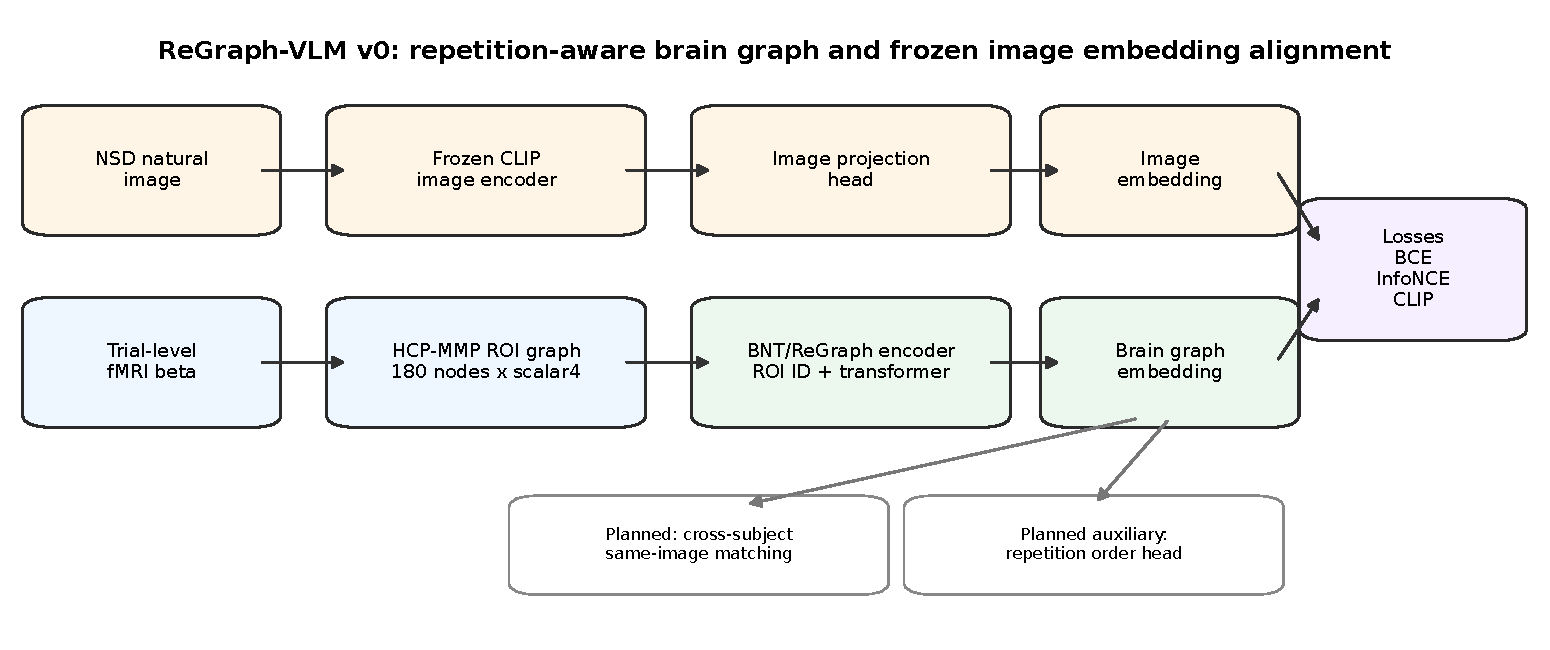
\includegraphics[width=0.98\linewidth]{figures/model_overview.pdf}
  \caption{ReGraph-VLM v0. Trial-level fMRI beta responses are converted into fixed-order 180-node ROI graphs. A BNT/ReGraph-style encoder maps each graph to a brain embedding. A frozen CLIP image encoder provides an image embedding target. Completed losses include pairwise BCE, repeat InfoNCE, and CLIP-style brain-image alignment. Cross-subject matching and repetition-order modeling are planned but not yet completed.}
  \label{fig:model}
\end{figure}

\section{Data and Graph Construction}

\paragraph{Atlas ROI graph.}
We pivoted from learned shared-unit graphs to atlas ROI graphs. Each node is one HCP-MMP cortical parcel, yielding 180 fixed-order nodes. This fixed node order is important: unlike generic graphs, ROI identity is anatomically meaningful, so readouts that destroy ROI position can fail.

\paragraph{Node features.}
For each ROI and trial-level beta response, we compute four scalar features:
\begin{equation}
  X_i = [\mathrm{mean\ beta},\ \mathrm{std\ beta},\ q90\ \mathrm{beta},\ \mathrm{positive\ fraction}].
\end{equation}
This feature set is intentionally simple. It allowed stable dataset construction and produced a strong ROI MLP sanity baseline.

\paragraph{Strict T=3 repetition dataset.}
We use strict three-repeat sequences, so each usable sample contains $(G_{s,i,1}, G_{s,i,2}, G_{s,i,3})$. The initial smoke folds are \texttt{fold\_01} and \texttt{fold\_04}. Previous dataset QC confirmed that strict T=3 is feasible, that trial-level scalar4 caches are valid, and that NaN/Inf counts are zero. The first modeling target is same-image repeat matching: positives pair repeated graphs from the same subject and image; negatives are same-subject and repeat-pair matched but use different images.

\section{Completed Neuroscience Analyses}

Before training graph models, we tested whether repetition/familiarity signals are present in the ROI graphs. Figure~\ref{fig:neuro} summarizes the completed analyses.

\begin{figure}[t]
  \centering
  
\includegraphics[width=0.98\linewidth]{figures/neuroscience_summary.pdf}
  \caption{Completed neuroscience results. Left: number of ROIs with FDR-significant repeat effects. Middle: same-image repeated graphs are more similar than different-image controls across all repeat pairs. Right: schematic of the 180-node ROI graph, emphasizing the current interpretation: global graph structure remains stable while local repeat-sensitive edges exist. The right panel is schematic, not a cortical surface rendering.}
  \label{fig:neuro}
\end{figure}

\paragraph{ROI repetition effects.}
Repeated viewing produced measurable ROI-level changes. We found 41 FDR-significant ROIs for repeat2-repeat1 and 56 FDR-significant ROIs for repeat3-repeat1. The mean absolute real effects were much larger than shuffled-repeat controls: 10.90 versus 2.56 for repeat2-repeat1, and 14.33 versus 2.48 for repeat3-repeat1. This supports the claim that trial-level ROI responses change systematically across repeated viewing, consistent with repetition suppression/enhancement phenomena \citep{grill2006repetition}.

\paragraph{Same-image representational stability.}
Same-image repeated graphs were consistently more similar than different-image controls. For repeat pairs 1-2, 1-3, and 2-3, same-image correlations were 0.8916, 0.8851, and 0.8871, respectively, compared with different-image correlations of 0.8305, 0.8296, and 0.8292. The same-minus-different gaps were therefore 0.0612, 0.0555, and 0.0579.

\paragraph{Graph reconfiguration.}
Repeat-specific ROI correlation matrices were globally stable across repetitions, but local edge-level changes existed. Train-only fold-consistent edge analysis found 9 repeat-sensitive edges, including 3 fold-consistent repeat2-repeat1 edges and 6 repeat3-repeat1 edges. We interpret this conservatively: repeated viewing does not globally rewire the ROI graph, but local edge changes may carry repetition information.

\section{Models}

\paragraph{Raw and non-graph baselines.}
The raw baseline scores pairs using Pearson correlation over flattened ROI features. The strongest non-graph learned baseline is a Siamese ROI MLP trained with BCE+InfoNCE. This baseline is important because it preserves fixed ROI order through flattening and directly optimizes repeat matching.

\paragraph{Graph baselines.}
We tested GCN, GAT, BrainGNN \citep{li2021braingnn}, and Brain Network Transformer (BNT) \citep{kan2022bnt}. Naive GCN and BrainGNN collapsed in the pair-retrieval setting. This does not imply that graph structure is useless; rather, standard graph pooling can destroy fixed anatomical ROI identity. BNT-token with ROI identity and flatten readout was much stronger than BrainGNN and competitive with the ROI MLP.

\paragraph{ReGraph-VLM v0.}
ReGraph-VLM v0 uses the best BNT-token graph encoder as the brain branch and a frozen CLIP image encoder \citep{radford2021clip} as the image branch. The training objective combines pairwise BCE, repeat InfoNCE \citep{oord2018infonce}, and CLIP-style brain-image contrastive alignment:
\begin{equation}
  \mathcal{L} = \mathcal{L}_{\mathrm{BCE}} + \mathcal{L}_{\mathrm{repeat\ InfoNCE}} + \lambda_{\mathrm{clip}}\mathcal{L}_{\mathrm{CLIP}}.
\end{equation}
We tested $\lambda_{\mathrm{clip}}$ values and found $\lambda_{\mathrm{clip}}=2.0$ to be a stable current setting.

\section{Completed Results}

\subsection{Within-subject same-image repeat matching}

Table~\ref{tab:within_subject} reports the completed within-subject repeat-matching results. The main result is a tradeoff: ROI MLP variants are stronger for binary same/different discrimination, while BNT/ReGraph variants are competitive on retrieval-style metrics.

\begin{table}[t]
  \centering
  \caption{Completed within-subject same-image repeat matching results. Values are means over the available smoke folds and seeds for each experiment.}
  \label{tab:within_subject}
  \small
  \begin{tabular}{lcccc}
    \toprule
    Model & AUROC & AUPRC & R@5 & MRR \\
    \midrule
    Raw Pearson flat & 0.6182 & -- & 0.0522 & 0.0433 \\
    ROI MLP + BCE & 0.7672 & 0.7336 & 0.0543 & 0.0442 \\
    ROI MLP + BCE+InfoNCE & \textbf{0.7778} & \textbf{0.7540} & \textbf{0.0758} & \textbf{0.0592} \\
    Naive GCN & 0.5000 & -- & -- & -- \\
    BrainGNN Siamese & 0.5000 & -- & -- & -- \\
    BNT-token + BCE+InfoNCE & 0.7693 & 0.7512 & 0.0718 & 0.0584 \\
    \bottomrule
  \end{tabular}
\end{table}

\subsection{Graph-VLM alignment}

Adding CLIP alignment substantially improved brain-image retrieval compared with graph-only BNT/ReGraph. At $\lambda_{\mathrm{clip}}=2.0$, ReGraph-VLM was competitive with ROI-MLP+CLIP. ROI-MLP+CLIP slightly improved binary AUROC/AUPRC, while ReGraph-VLM slightly improved repeat-retrieval R@5/MRR and brain-to-image MRR (Table~\ref{tab:vlm}).

\begin{table}[t]
  \centering
  \caption{Completed ReGraph-VLM v0 comparison at $\lambda_{\mathrm{clip}}=2.0$ (six runs: two folds and three seeds).}
  \label{tab:vlm}
  \small
  \begin{tabular}{lcccccc}
    \toprule
    Model & AUROC & AUPRC & R@5 & MRR & Image R@5 & Brain MRR \\
    \midrule
    ROI-MLP+CLIP & \textbf{0.7710} & \textbf{0.7411} & 0.0568 & 0.0475 & 0.0625 & 0.0563 \\
    BNT/ReGraph+CLIP & 0.7673 & 0.7402 & \textbf{0.0602} & \textbf{0.0503} & 0.0625 & \textbf{0.0596} \\
    \bottomrule
  \end{tabular}
\end{table}

\subsection{Hard-negative stress test}

We also trained with a mixed negative set: 50\% random matched negatives and 50\% top-10\% Pearson hard negatives. This made binary discrimination harder. ROI-MLP+CLIP retained higher AUROC/AUPRC, but BNT/ReGraph+CLIP slightly improved retrieval and brain-alignment metrics (Table~\ref{tab:hardneg}).

\begin{table}[t]
  \centering
  \caption{Completed hard-negative stress test at $\lambda_{\mathrm{clip}}=2.0$.}
  \label{tab:hardneg}
  \small
  \begin{tabular}{lcccccc}
    \toprule
    Model & Hard AUROC & Hard AUPRC & Hard R@5 & Hard MRR & Brain R@5 & Brain MRR \\
    \midrule
    ROI-MLP+CLIP & \textbf{0.6965} & \textbf{0.6583} & 0.0536 & 0.0469 & 0.0577 & 0.0520 \\
    BNT/ReGraph+CLIP & 0.6730 & 0.6492 & \textbf{0.0562} & \textbf{0.0478} & \textbf{0.0699} & \textbf{0.0567} \\
    \bottomrule
  \end{tabular}
\end{table}

\begin{figure}[t]
  \centering
  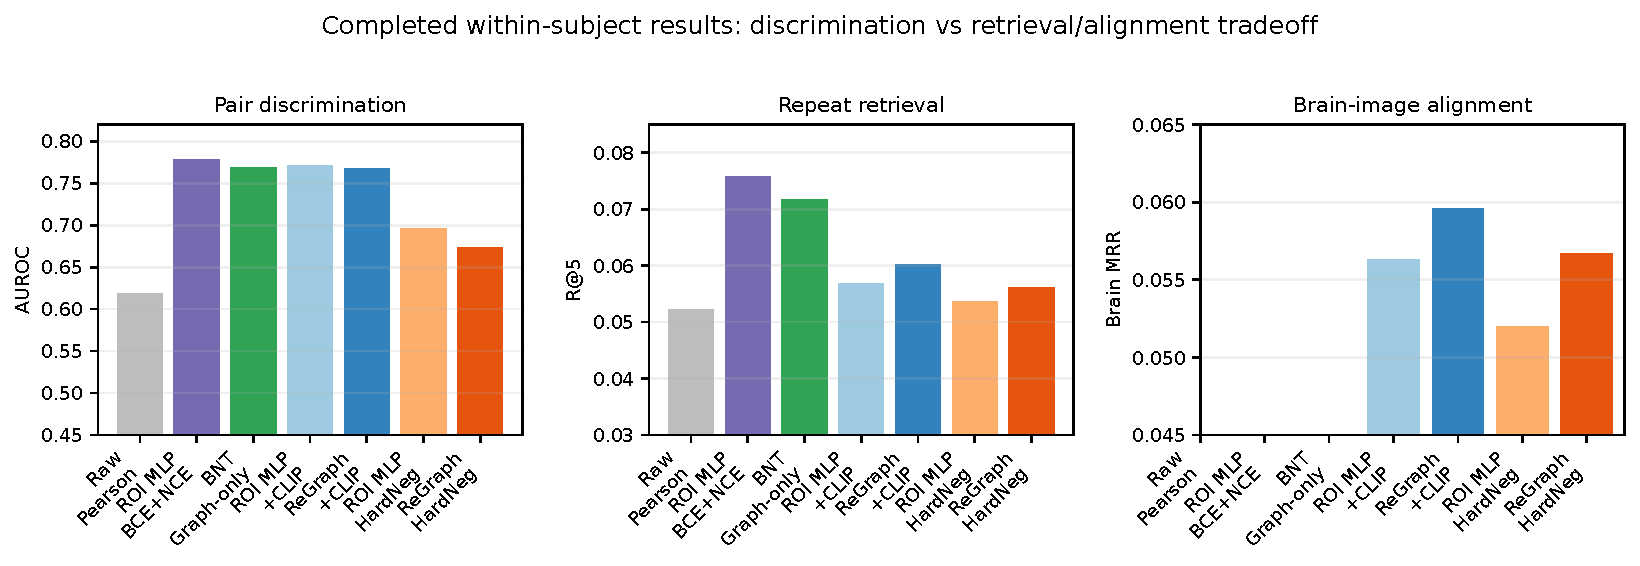
\includegraphics[width=0.98\linewidth]{figures/results_tradeoff.pdf}
  \caption{Completed model results show a stable tradeoff. ROI MLP variants are stronger for binary discrimination, while graph-VLM variants are more competitive on retrieval/alignment metrics.}
  \label{fig:results}
\end{figure}

\section{Pending Experiments From the Proposal}

\subsection{Cross-subject same-image matching}

\paragraph{Status.}
Pending. Jobs for the first cross-subject wave have been prepared/submitted, but the final dataset QC and model summaries are not yet available. Therefore, no cross-subject numbers are reported here.

\paragraph{Planned protocol.}
The next task is held-out-subject same-image matching. Positives pair the same image across different subjects with matched repeat index. Negatives pair different images across different subjects with matched repeat index. The main evaluation is retrieval: given a held-out subject brain graph, retrieve the matching image/reference graph from training-subject candidates.

\begin{table}[h]
  \centering
  \caption{Cross-subject matching results are intentionally left blank until the jobs complete.}
  \small
  \begin{tabular}{lcccc}
    \toprule
    Model & AUROC & R@5 & MRR & Status \\
    \midrule
    Raw Pearson & -- & -- & -- & Pending \\
    ROI-MLP+CLIP & -- & -- & -- & Pending \\
    BNT/ReGraph & -- & -- & -- & Pending \\
    BNT/ReGraph+CLIP & -- & -- & -- & Pending \\
    \bottomrule
  \end{tabular}
\end{table}

\subsection{Auxiliary repetition-order learning}

\paragraph{Status.}
Planned auxiliary task only. No order-learning dataset or model results are reported here.

\paragraph{Motivation.}
Single-graph repeat-index classification is heavily confounded by session/order structure. Therefore, the better auxiliary task is not ordinary repeat1/repeat2/repeat3 classification. Instead, we plan controlled same-image order tasks that hold subject and image fixed.

\paragraph{Planned tasks.}
First, pairwise repetition direction asks whether, for two graphs from the same subject-image sequence, the second graph came later. Second, sequence order verification asks whether a three-graph sequence is in the true order $[G_1,G_2,G_3]$ or a shuffled order. Third, ordinal repeat embedding learns a score $o(G)$ such that $o(G_{s,i,1}) < o(G_{s,i,2}) < o(G_{s,i,3})$.

\paragraph{Planned controls.}
The auxiliary task will require session-only baselines, within-subject repeat-label shuffles, different-image controls, and optionally session-residualized features. Without these controls, order prediction could reflect session drift rather than image-specific repetition dynamics.

\section{Discussion}

The completed project has three stable conclusions. First, repetition/familiarity effects are measurable in trial-level HCP-MMP ROI graphs: ROI activity changes across repeats, same-image graphs remain more similar than different-image controls, and local edge changes exist despite globally stable ROI correlation structure. Second, same-image repeat matching is learnable: a contrastive ROI MLP improves substantially over raw ROI-pattern similarity. Third, existing off-the-shelf graph baselines are not automatically suitable for this task. Naive GCN and BrainGNN collapse in the Siamese setting, while BNT-token with fixed ROI order is competitive but does not clearly beat the ROI MLP.

ReGraph-VLM v0 gives a more specific result. Frozen CLIP alignment improves image-brain retrieval compared with graph-only BNT/ReGraph. However, the model is not yet a decisive win over ROI-MLP+CLIP. The honest current interpretation is that ROI-MLP+CLIP is stronger for binary same/different discrimination, whereas BNT/ReGraph+CLIP is more competitive for retrieval-style and brain-image alignment metrics. This is why the next completed experiment should be cross-subject same-image matching: if graph-VLM structure is useful, its advantage should become clearer in the harder subject-invariant retrieval setting.

\section{Conclusion}

We built a repetition/familiarity graph-learning pipeline for NSD trial-level fMRI using 180-node HCP-MMP ROI graphs. Completed neuroscience analyses establish repetition modulation, same-image stability, and subtle graph reconfiguration. Completed modeling results show that contrastive learning is essential and that CLIP alignment improves brain-image retrieval. The remaining report sections are deliberately left pending where experiments are not yet complete: cross-subject same-image matching and auxiliary repetition-order learning. These are the next tests needed to determine whether ReGraph-VLM can move from a competitive within-subject model to a stronger subject-invariant brain graph and vision alignment framework.

\bibliographystyle{plainnat}
\bibliography{references}

\end{document}
